\documentclass{article}

\usepackage{physics} % Handy shortcuts like \pdv, \dd and much more
\usepackage{geometry} % smaller margins, can be adjusted if given arguments
\usepackage{siunitx} % the \si environment for units
\usepackage{mathtools} % The dcases environment, prettier than just cases
\usepackage{tikz} % For drawing picures
\usepackage{wrapfig} % Wrapping text around figures


\title{Exercise 3 - TFY4345 Classical Mechanics}
\date{2020}

\begin{document}
    \maketitle
    \section{Pendulum on spinning a wheel}
    \begin{wrapfigure}{r}{0.25\textwidth}
        \vspace{-1cm}
        \includegraphics[width=0.25\textwidth]{figures/figure_1.pdf}
        \vspace{-2cm}
    \end{wrapfigure}
    The point of support of a simple pendulum of length $b$ moves on a massless rim of radius $a$, rotating with a constant angular velocity $\omega$. Obtain the expression for the Cartesian components of the velocity and acceleration for the mass $m$. Obtain also the angular acceleration for the angle $\theta$, shown in the figure, by using Euler's equation.
    \vspace{1cm}

    \section{Bead on a ring}
    \begin{wrapfigure}{2}{0.25\textwidth}
        \vspace{-1.5cm}
        \includegraphics[width=0.25\textwidth]{figures/figure_2.pdf}
        \vspace{-2cm}
    \end{wrapfigure}
    A bead is attached to a ring with radius $R$ where it can slide frictionless. The ring itself is attached to a vertical shaft which rotates with a constant angular velocity (let us assume that the shaft does not affect the bead motion). Obtain by using the Euler equations the equilibrium position of the bead.
    \vspace{1cm}

    \section{Atwood's machine}
    \begin{wrapfigure}{r}{0.25\textwidth}
        \vspace{-1cm}
        \includegraphics[width=0.25\textwidth]{figures/figure_3.pdf}
        \vspace{-2cm}
    \end{wrapfigure}
    Determine the Hamiltonian and Hamilton's equations of motion for a s simple Atwood's machine (one pulley), as shown in the figure. The pulley radius i $a$ and the moment of inertia $I$.
    \newpage

    \section{Particle on a moving wedge}
    \begin{wrapfigure}{r}{0.35\textwidth}
        \vspace{-1cm}
        \includegraphics[width=0.35\textwidth]{figures/figure_4.pdf}
    \end{wrapfigure}
    A particle of mass $m$ slides down a smooth, circular wedge of mass $M$ as shown in the figure. The wedge rests on a smooth, horizontal table with coordinate $x$. \\ \\
    (a) Find the equation of motion $m$ and $M$. \\ \\
    (b) Find the reaction of the wedge on $m$, as a function of $\theta$ and it's derivatives. \\ \\
    (Note: This one is tedious, focus on the 3 others first) \\ 
    (Hint: Use the method of Lagrange's undetermined multiplier. Select $x$ and $\theta$ as generalized coordinates.)


\end{document}
